\section{Installation}

%%%%%%%%%%%%%%%%%%%%%%%%%%%%%%%%%%%%%%%%%%%%%%%%%%%%%%%%%%%%%%%%%%%%%%%%%%%%%%%%

\begin{frame}[fragile]{Architecture}

\begin{figure}
\begin{center}
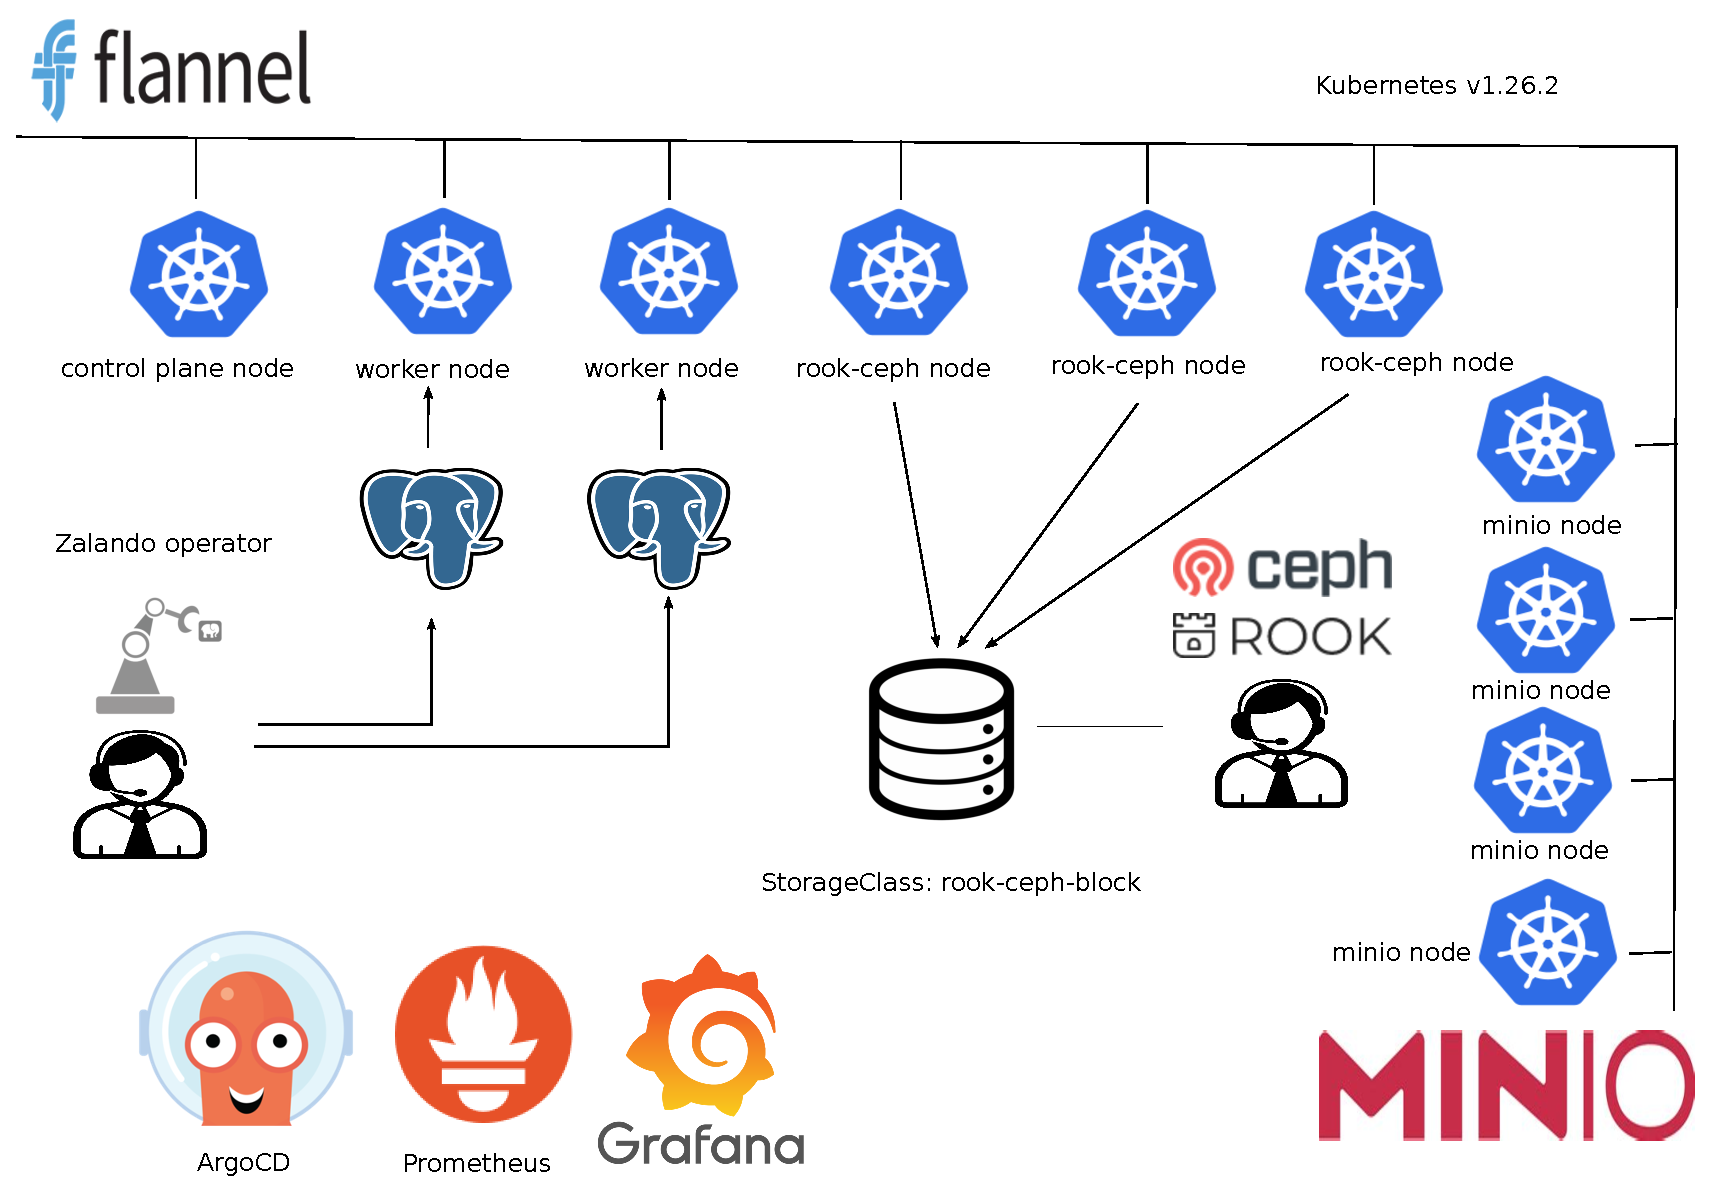
\includegraphics[angle=0, width=0.5\textwidth]{images/architecture.eps}
\end{center}
\end{figure}

\end{frame}

%%%%%%%%%%%%%%%%%%%%%%%%%%%%%%%%%%%%%%%%%%%%%%%%%%%%%%%%%%%%%%%%%%%%%%%%%%%%%%%%

\begin{frame}[fragile]{Versions utilisées}

   \begin{itemize}
      \item OS de déploiement: Debian 11 - Bullseye
      \item Versions de Kubernetes: 1.26.x
   \end{itemize}

\end{frame}

%%%%%%%%%%%%%%%%%%%%%%%%%%%%%%%%%%%%%%%%%%%%%%%%%%%%%%%%%%%%%%%%%%%%%%%%%%%%%%%%

\begin{frame}[fragile]{Déploiement du n{\oe}ud \textbf{control plane}}

   Kubernetes s'appuie sur un élément essentiel qui est le \textit{container runtime}.
   La méthode de déploiement du container runtime s'appuie la méthode décrite dans le lien: https://docs.docker.com/engine/install/debian/

\end{frame}

%%%%%%%%%%%%%%%%%%%%%%%%%%%%%%%%%%%%%%%%%%%%%%%%%%%%%%%%%%%%%%%%%%%%%%%%%%%%%%%%

\begin{frame}[fragile]{Déploiement du n{\oe}ud \textbf{worker}}

TODO

\end{frame}

%%%%%%%%%%%%%%%%%%%%%%%%%%%%%%%%%%%%%%%%%%%%%%%%%%%%%%%%%%%%%%%%%%%%%%%%%%%%%%%%

\begin{frame}[fragile]{Déploiement de la couche réseau - \textbf{Container Network Interface}}

TODO

\end{frame}

%%%%%%%%%%%%%%%%%%%%%%%%%%%%%%%%%%%%%%%%%%%%%%%%%%%%%%%%%%%%%%%%%%%%%%%%%%%%%%%%

\begin{frame}[fragile]{Déploiement du stockage - \textbf{Rook Ceph}}

\begin{tiny}
\begin{Verbatim}[commandchars=\\\{\}]
linagora@debian-cp:~$ kubectl get storageclass
NAME              PROVISIONER                    RECLAIMPOLICY   VOLUMEBINDINGMODE      ALLOWVOLUMEEXPANSION   AGE
local-storage     kubernetes.io/no-provisioner   Delete          WaitForFirstConsumer   false                  12d
rook-ceph-block   rook-ceph.rbd.csi.ceph.com     Delete          Immediate              true                   5d23h
\end{Verbatim}
\end{tiny}

\end{frame}

%%%%%%%%%%%%%%%%%%%%%%%%%%%%%%%%%%%%%%%%%%%%%%%%%%%%%%%%%%%%%%%%%%%%%%%%%%%%%%%%

\begin{frame}[fragile]{Déploiement de l'opérateur \textbf{PostgreSQL} de Zalando}

TODO

\end{frame}

%%%%%%%%%%%%%%%%%%%%%%%%%%%%%%%%%%%%%%%%%%%%%%%%%%%%%%%%%%%%%%%%%%%%%%%%%%%%%%%%

\begin{frame}[fragile]{Répartitions des pods \textbf{PostgreSQL} sur les n{\oe}uds worker}

TODO

\end{frame}

%%%%%%%%%%%%%%%%%%%%%%%%%%%%%%%%%%%%%%%%%%%%%%%%%%%%%%%%%%%%%%%%%%%%%%%%%%%%%%%%
